\documentclass[11pt,letterpaper]{article}
\usepackage{array}
\usepackage[in]{fullpage}
\usepackage{verbatim}
\usepackage{parskip}
\usepackage{graphicx}

\usepackage{titlesec}
\titlespacing{\section}{0pt}{\baselineskip}{0pt}
\titleformat*{\section}{\normalsize\bfseries\MakeUppercase}

\titlespacing{\subsection}{0pt}{0.5\baselineskip}{0pt}
\titleformat*{\subsection}{\normalsize\bfseries}

\titlespacing{\subsubsection}{0pt}{0.5\baselineskip}{0pt}
\titleformat*{\subsubsection}{\normalsize\bfseries}

%\setlength{\parindent}{0in}

\begin{document}
\setlength{\parindent}{0in}
%\baselineskip 4pt
\newcommand{\tablespace}[0]{\vspace{8pt}}
\textbf{ENVS S422: Earth's Climate System\\
Modeling Exercise 4: A highly simplified model of thermohaline circulation}\\%\footnote{Based on exercises developed by Dave Bice at Penn State University.}}\\

The atmosphere and the ocean transport heat from the equator to the poles. In this exercise you will investigate thermohaline circulation of the ocean in a model that has more than one steady state (the model is based on the work of Stommel, 1961). Ocean circulation is determined by density gradients between the tropics and the poles, which are themselves functions of temperature and salinity. You will investigate changes in thermohaline circulation in response to various perturbations to the steady-state solutions.

For each model experiment, you should submit a brief 1-paragraph response to the questions that are being explored in the exercise and \textit{at least} one graph to help justify your response.

Due date: 4 March 2019

\section{Model description}
This modeling exercise is based on the classic 2-box model of Stommel (1961). The model consists of a ``polar box'' with cold, relatively fresh water, and an ``equatorial box'' that contains warm, salty water. Water flows from the surface of the equatorial box to the surface of the polar box (like the Gulf Stream). When it reaches the polar box it cools, densifies, and sinks. Eventually the water leaves from the bottom of the polar box and travels as a deep flow back to the equatorial box (like the North Atlantic Deep Water).



The model derivation is quite complicated and beyond our interests here, which is to explore steady-state flow of a system. Note that the equations that we'll use have been ``non-dimensionalized'' for numerical reasons. 

The first thing we need are equations describing the transport of heat (i.e., temperature) and salinity. We will approximate the heat transport by
\begin{equation}
\frac{d\Delta{T}}{dt}=\Delta{T_{eq}}-\Delta{T}-Q\Delta{T},
\label{eq:deltaT}
\end{equation}
where $\Delta{T}$ is the temperature difference between the boxes, $Q$ is the flow between the boxes, and $\Delta{T_{eq}}=1$ is the equilibrium temperature difference (in non-dimensional temperature units) that the system would achieve if $Q=0$ (i.e., if thermohaline circulation is shut off). The reason that $\Delta{T_{eq}}$ is not equal to zero is that the equator tends to absorb heat whereas the poles tend to lose heat. This ensures that there is a temperature gradient in the absence of circulation.

The $\Delta{T}$ term (by itself) represents heat conduction through the water. Even if the water doesn't flow there will be some transport of heat from the equator to the poles. The $Q\Delta{T}$ terms represents heat advection (i.e., physical transport of heat by the ocean currents). The negative signs in front of these terms indicate negative feedbacks: fast currents and large temperature gradients tend to cause the temperature gradients to decrease.

Equation (\ref{eq:deltaT}) may be easier to understand by considering how the temperature profile varies with latitude (Fig. \ref{fig:T_gradient}). Essentially, the model is trying to evolve toward a steady-state temperature profile, which is given by
\begin{equation}
\Delta{T}=\frac{\Delta T_{eq}}{1+Q}.
\end{equation}
Equation (\ref{eq:deltaT}) thus describes the rate at which the system evolves toward the equilibrium profile. If the flow $Q$ is constant, then this exercise becomes straightforward --- $\Delta T$ decays exponentially until it equals $\Delta T_{eq}/(1+Q)$. However, in general $Q$ is not constant and in fact depends on both temperature and salinity differences.

\begin{figure}[t]
\begin{center}
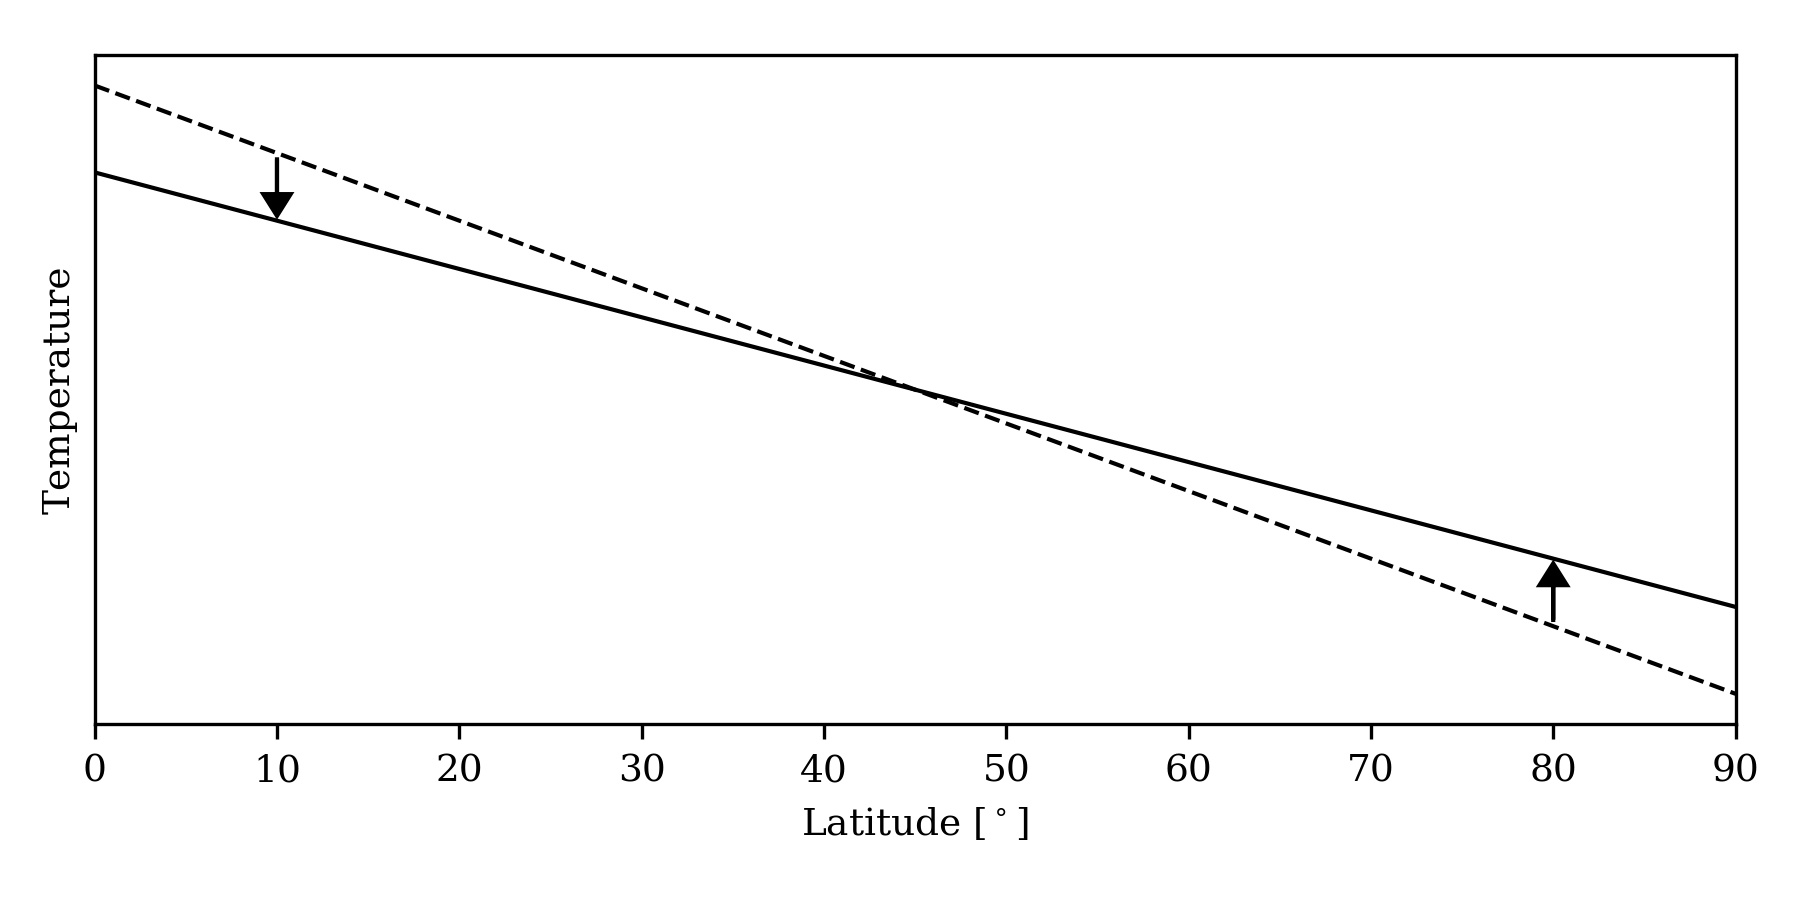
\includegraphics[]{./T_gradient.jpg}
\end{center}
\caption{Schematic of meridional temperature profile at some time $t$ (dashed line) and the equilibrium/steady-state temperature profile (solid line). The system continuously tries to evolve toward the equilibrium profile. If thermohaline circulation is shut off, then the equilibrium profile $T_{eq}$, otherwise its $T_{eq}/(1+Q)$.}
\label{fig:T_gradient}
\end{figure}

\begin{figure}[h]
\begin{center}
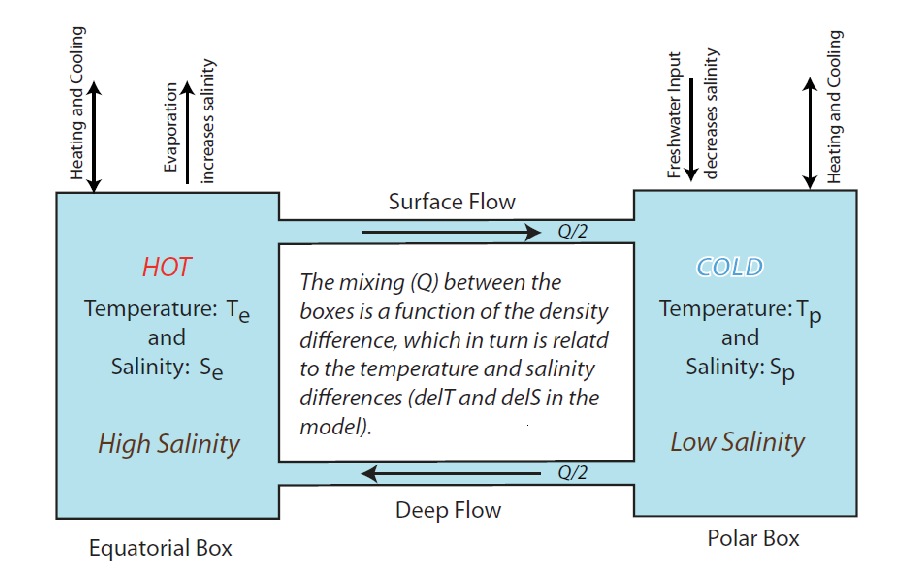
\includegraphics[]{./fig1}
\caption{Schematic diagram of the simple thermohaline circulation model that you will explore.}
\end{center}
\end{figure}

We will use a similar equation for modeling ocean salinity, by setting
\begin{equation}
\frac{d\Delta{S}}{dt}=\delta(\Delta{S_{eq}}-\Delta{S})-Q\Delta{S},
\label{eq:deltaS}
\end{equation}
where $\Delta{S}$ is the salinity difference between the boxes, $\Delta{S_{eq}}$ is the salinity difference that the system would achieve if $Q=0$, and $\delta<{1}$ is a scaling constant that causes salt diffusion to occur more slowly than heat conduction. In other words, changes in temperature occur more quickly than changes in salinity. All other aspects of this equation are identical to the temperature equation.

The flow of water through the system is governed by
\begin{equation}
Q=\frac{\Delta{\rho}}{\lambda},
\end{equation}
where $\Delta{\rho}$ is the density difference between the boxes (large $\Delta{\rho}$ causes fast currents) and $\lambda$ is a non-dimensional number --- think of it as resistance to flow. If $\lambda$ is large, the ocean currents will be small.

Finally, we need an equation to describe the density difference between the two boxes, which depends on the salinity and temperature differences:
\begin{equation}
\Delta{\rho}=|R\Delta{S}-\Delta{T}|,
\label{eq:rho}
\end{equation}
where $R$ is a constant, which is used to modify the importance of salinity relative to temperature. This equation requires some explanation:
\begin{itemize}
\item The salinity difference and temperature differences, $\Delta S$ and $\Delta T$, are both greater than 0 because water at the equator is both hotter and saltier than water at the poles.
\item Salinity and temperature have opposing effects on density, in that density increases with increasing salinity but decreases with increasing temperature.
\item In other words, the negative sign in Equation (\ref{eq:rho}) occurs because the salinity difference acts to reduce the density difference whereas the temperature difference acts to increase the density difference.
\item Finally, the $\Delta S$ and $\Delta T$ are defined as the the salinity and temperature at the equator minus the salinity and temperature at the poles, respectively, both of which are positive values. However, the density difference, $\rho_{equator}-\rho_{pole}$, is generally negative because the water at the pole is more dense than the water at the equator. The absolute value sign ensures that the flow remains positive (from the equator to the poles) by forcing the density difference to be positive.
\end{itemize}


This is an elegant, but kind of strange, way to formulate a model of thermohaline circulation. Instead of creating reservoirs to represent ocean temperature and salinity, we will construct reservoirs to represent temperature and salinity \textit{differences}. Those temperature and salinity differences will determine density differences, and it is those density differences that drive flow. Furthermore, we've represented the surface currents and deep currents by a single equation (we can do this because the currents must be related through mass conservation). The temperature and salinity differences will evolve as the water flows between reservoirs. Finally, we've accounted for freshening and cooling of the polar box and heating and evaporation of the equatorial box by forcing the temperature and salinity differences to increase in the absence of circulation. 


\section{Experiments}
\subsection{Preliminary experiment}
Download the STELLA thermohaline circulation model from blackboard. The model consists of two reservoirs, deltaT and deltaS, that represent temperature and salinity differences between the tropics and the poles. Each of these reservoirs is connected to a single biflow that can increase or decrease the temperature and salinity differences. Set the model to run from 0 to 15 (time units are scaled to the diffusional time scale of the system, which is thought to be about 200 years), with DT=0.01, using the Runge‐Kutta 2 method. Run the model.

Make a plot showing how the temperature difference deltaT, salinity difference deltaS, and flow Q change with time. How long does it take the system to evolve to a steady state? You can think of Q as the combined flow of the Gulf Stream and the North Atlantic Deep Water and is designed to be greater than or equal to 0. Q only indicates the magnitude of the flow, not the direction. Based on your observations from this preliminary experiment, describe the relationship between deltaT, deltaS, and Q.


\subsection{Varying the initial reservoir values}
Now investigate the impact that the initial reservoir values have on the model solutions.

(a) Change the deltaS initial value from 0.5 to 0. Before running the model, take note of the steady state values of deltaS, deltaT, and Q from the preliminary experiment. Then, run the model and see what happens. How did this simulation differ from the preliminary experiment? Why?

(b) Now explore a wider range of initial values to better understand the steady states of this system. Go to the Sensi Specs window from the Run menu and send both reservoirs over to the selected column. Make 11 runs, and have deltaS go from 0 to 1 and deltaT go from 1 to 0; be sure to hit the Set button after you define the starting and ending values. Then set up a graph to view the results --- make it a comparative scatter plot, with deltaS on the x-axis and deltaT on the y-axis. Then run the model and observe what happens. You can watch the trajectory of each run by following the dots --- they move fast when the system is not in steady state, but they become stationary when a steady state is achieved. So if there is one steady state, all dots will converge on a single spot; if there are multiple steady states you’ll see more than one convergence. These convergences, also known as attractors, can be thought of as similar to topographic depressions. Imagine a topographic surface with some peaks and some depression; the depressions represent conditions where the two flows in our model are both zero. If you toss a bunch of marbles onto this smooth surface, they will tend to find their way to the depressions, and the initial starting point of the marble determines which depression it ends up in.

Now, study the results of these model runs and find out how many steady states there are for this system (you may want to modify your sensitivity specs a bit to cover more of the space in the deltaS vs. deltaT plot) and then report the $\langle\Delta S, \Delta T\rangle$ coordinates of the steady states. For the following two exercises, which involve perturbations to the thermohaline circulation, it will be instructive to create plots of deltaT vs. deltaS.

\subsection{A warming climate}
What will happen to this system if the climate warms? How can we modify the system to represent a warmer climate? Recent climate change has been characterized by greater warming at high latitudes, which tends to reduce the gradient from the poles to the equator. In our model, the temperature difference between the polar and equatorial regions is represented by the deltaT reservoir. The value or magnitude of deltaT is a function of two things: the density-driven mixing that tends to even out the temperature difference (reducing deltaT) and the climate-controlled temperature difference (Teq in our model), which is set to 1. If we reduce Teq, that will tend to drive the system to a lower deltaT value.

Set Teq equal to time and make it a graphical function of time. Make the upper limit 1 and the lower limit 0.5 (anything lower would be too extreme). Set the time axis to go from 0 to 30 so that we can make the change in Teq after the system has gotten into a steady state (it would be hard to understand the effect of the change during the adjustment to steady state). So, after about 8 time units, make Teq step down to a lower value and then have it remain at that value for a brief period of time and then return it to 1. There are two questions to answer here:

(a) Working with the initial deltaT and deltaS settings of 0.5, how does the system respond to \textit{different} magnitudes and durations of the excursion of Teq? Does the system always bounce back to the original steady state, or can it get knocked into the other steady state? If it does get knocked into another steady state, is it one of the same steady states that we found earlier, by just changing the initial values of the reservoirs without tampering with Teq? In general, describe how this change affects the magnitude of deltaS, deltaT, and Q. This will require some careful analysis of the model parameters, but do your best to explain why the system behaves this way.

(b) You should have found previously that this system has two steady states. In (a), you tampered with one of the steady states. Now, let’s do the same kind of tampering with the other steady state. Set the initial value of delS to 0.25. Check that this gives you a different steady-state. Now, how does it react to the periods of decreased Teq? Is this steady state more sensitive or less sensitive to changes in Teq than the other steady state?

\subsection{Freshwater pulses}
The Younger-Dryas was a cooling period during the end of the last ice age that is believed to have been triggered by a change of state in the thermohaline circulation due to a pulse of freshwater added to the North Atlantic. Cessi (1994) figured out that the pulse of water in Stommel's model would represent a flux of 0.2 delS units for a period of between 3--5 time units. Find a way to modify your model to simulate this freshwater pulse. HINT: you want to add to the delS reservoir for a limited period of time, and you want to impose this on the steady state condition that represents the warmer (high Q and low delT) of the two steady states.

(a) Show how you make this change to your model (make a sketch, or print out the altered model), and then carry out the experiment. Does this pulse knock the system into the colder of the two steady states? In other words, does it stay in that other state even after the pulse of freshwater has ended? Again, delve into the inner workings of the model to understand what is going on.

(b) What is the \textit{minimum magnitude and duration} of freshwater pulse that is needed to knock the system into the other steady state?



\section{References}
Cessi, P., 1994, A simple box model of stochastically forced thermohaline flow, \textit{J. Phys. Oceanogr.}, 24, 1911--1920.

Stommel, H., 1961, Thermohaline convection with two stable regimes of flow, \textit{Tellus}, 13(2), 224--230.

\end{document}
